\documentclass[11pt,a4paper]{ivoa}
\input tthdefs

\title{Group Membership Service}

\ivoagroup{Grid and Web Services}

\author{Brian Major}
\author{Patrick Dowler}
\author{Giuliano Taffoni}
\author{Adrian Damian}
\author{Marco Molinaro}

\editor{Brian Major}

% \previousversion[????URL????]{????Funny Label????}
\previousversion{This is the first public release}

\begin{document}
\begin{abstract}

The Group Membership Service (GMS) specification describes a REST interface for determining whether a user is a member of a group.  This information can be used to protect access to proprietary resources: clients can issue a call to GMS when an authorization decision needs to be made.  Proprietary resources can be any number of things such as data, metadata or services.  Because a single group can be used to protect multiple resources, GMS enables the creation of groups that represent teams with common authorization rights.  GMS offers organizations an interoperable, flexible and scalable way of protecting a hetergenous set of resources.

\end{abstract}

\section*{Acknowledgments}

???? Or remove the section header ????

\section*{Conformance-related definitions}

The words ``MUST'', ``SHALL'', ``SHOULD'', ``MAY'', ``RECOMMENDED'', and
``OPTIONAL'' (in upper or lower case) used in this document are to be
interpreted as described in IETF standard RFC2119 \citep{std:RFC2119}.

The \emph{Virtual Observatory (VO)} is a
general term for a collection of federated resources that can be used
to conduct astronomical research, education, and outreach.
The \href{http://www.ivoa.net}{International
Virtual Observatory Alliance (IVOA)} is a global
collaboration of separately funded projects to develop standards and
infrastructure that enable VO applications.


\section{Introduction}

Through standard IVOA protocols, many astronomy data centres and institutes offer users access to datasets (DALI \citep{std:DALI}, Datalink \citep{std:Datalink}, etc), metadata (TAP \citep{std:TAP}) and storage (VOSpace \citep{std:VOSpace}).  In some cases this information is proprietary--it is only allowed to be accessed by certain individuals.  Due to the wide variety and inherently institute-specific set of rules that may define how the information is proprietary, it is beneficial to the owners and maintainers of the rules to have a standard way of describing who has access to what resources.  Additionally, the rules describing resource access may be determined by an entity external to the holder of these resources.  To these ends, this document sets out a standard, programatic, and interoperable method of determining whether a given user is allowed to access a given resource.

The ideas presented by GMS enable data centres to do authorization checks in an interoperable fashion.  In the context of authorization, interoperability can viewed on two levels:  interoperability amongst the cooperating services \emph{within} a data centre, and interoperability \emph{between} data centres.  Because of the orthogonal nature of authorization, these levels amount to the same problem.

Interoperability aside, GMS describes a simple, general, maintainable, and scalable approach to performing authorization, and so is a recommended architectural pattern for managing access to proprietary resources.

\subsection{Proprietary resources}

Most facilities have a period of time in which only the Principal Investigator's team has access to observation metadata and data files.  Even without a proprietary period, time is required to verify and validate observations before they can be made public.

Projects also frequently create higher level products such as catalogs and images.  When these products are stored in a data centre, they must be accessible to only those who are authorized.

Proprietary information exists.  For it to be made available in a data centre to those with authorization, a way of performing that authorization check is required.

\subsection{Role within the VO Architecture}

\begin{figure}
\centering

% Get the architecture diagram from the TCG chair
% http://wiki.ivoa.net/twiki/bin/view/IVOA/IvoaTCG
% If they give you a PDF, for now dumb it down to a png by
% convert -antialias -density 72x72 archdiag.pdf archdiag.png
% Oh -- Notes don't need this; you'd have to remove archdiag.png
% from FIGURES in the Makefile, too.

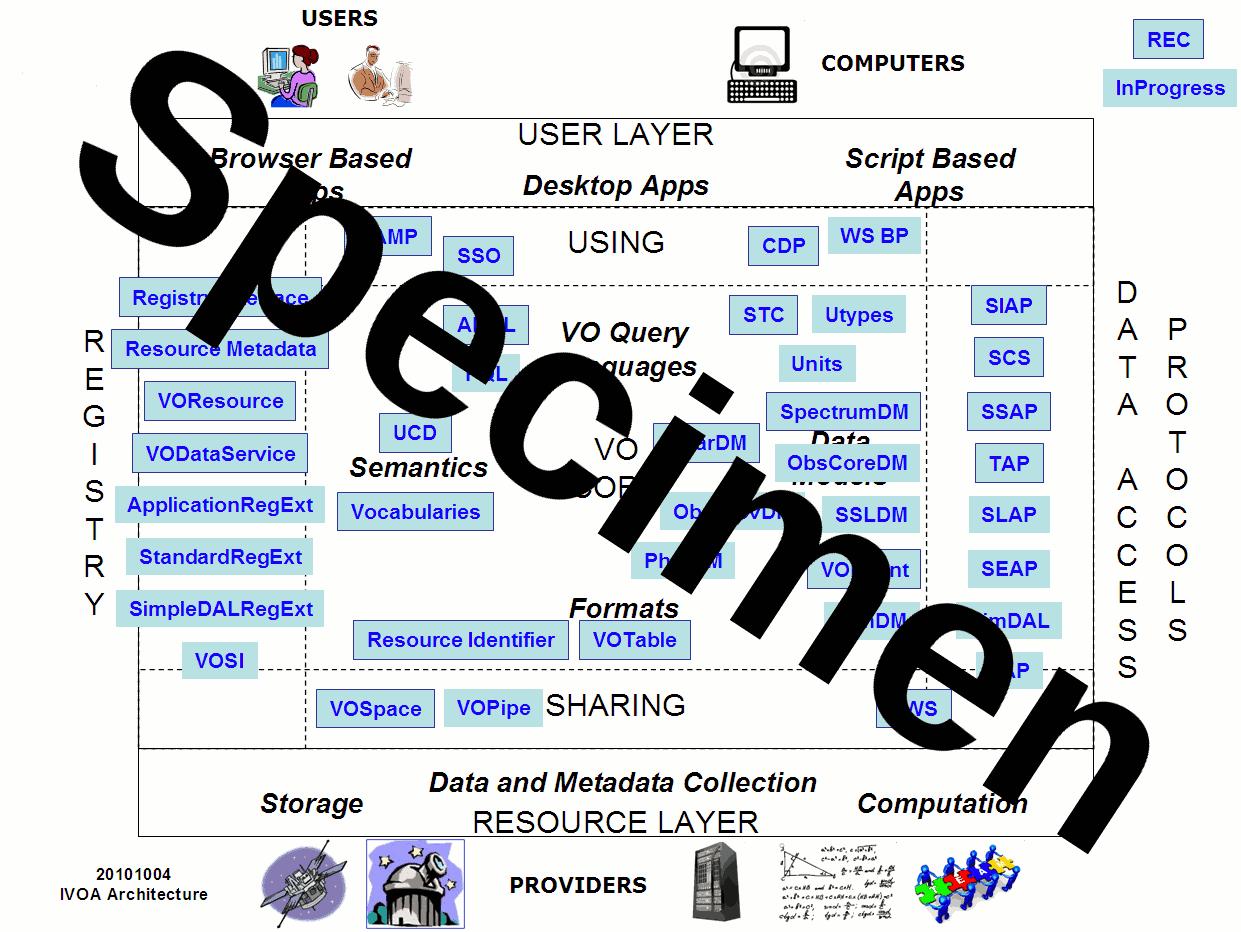
\includegraphics[width=0.9\textwidth]{archdiag.png}
\caption{Architecture diagram for this document}
\label{fig:archdiag}
\end{figure}

Fig.~\ref{fig:archdiag} shows the role this document plays within the
IVOA architecture \citep{note:VOARCH}.

GMS can be used by any software that needs to check, for authorization purposes, whether a user is a member of group.  Because of this general use case, GMS cuts through all of the IVOA and lies squarely in the middle of the SHARING technical resource in the IVOA architecture diagram.

\subsection{Use Cases}

Asside from the main use case of restricting access to proprietary resources, GMS supports a number of other use cases, of both the user and system variety.

\paragraph{Proprietary information} Restricting access to proprietary resources to certain users.

\paragraph{Homogeneity} Using the same mechanism to control access to proprietary resources in a data centre or in multiple data centres.

\paragraph{Scalability} A distributed mechanism that scales linearly with the resources being protected.

\paragraph{Remotely managing access} A project may wish to control access to resources that reside externally.

\paragraph{Access rule sharing} A project may consist of a variety of resources that can be all managed by the same access rules.

\paragraph{Extending the services of a data centre} A project that has hosted data and metadata at a data centre may wish to create value-added services outside of the data centre itself.  If some of the data or metadata is proprietary, the extended services may need to determine if a user is allowed to perform certain action on that data or metadata.

\paragraph{Cooperating institutes} Two or more institutes may work together on a single project that involves proprietary resources so require a common mechanism for protecting those resources.

\subsection{Definitions}

\paragraph{Authentication} User identification through credentials or identity provider.  See IVOA Single-Sign-On Profile: Authentication Mechanisms.  \citep{std:SSOAUTH}

\paragraph{Authorization} Making the decision of whether to grant a user permission to a given resource.  The decision can involve knowing the user's identity.

\paragraph{Resource} Something that may require authorization for access.  For example, a service, a data file, metadata.

\paragraph{User} An individual identified by authentication.

\paragraph{Group} A set of users.

\paragraph{Grant} Authorizing access to a protected resource by assigning a group.

\paragraph{Revoke} Removing access to a protected resource by removing an assigned group.

\paragraph{Owner} A user or group of users who may grant or revoke access to a specific resource.

\section{Authorization Requirements}

When looking at a system that has proprietary resources that need to be protected, it is clear that there are two distinct phases to authorization:  the assignment of the rules protecting the resources, and the attempts by various users to gain access to those resources.  They are described here:

\begin{enumerate}
\item The owner(s) of a resource may, at any time, change the rules by which a resource may be accessed. This is the \emph{granting and revoking of access}.
\item When users try to access resources, the granting rules for that resource are evaluated at runtime. This is the \emph{authorization check}.
\end{enumerate}

With these phases in mind and with the use cases defined, we can state that the goals of authorization are to:

\begin{itemize}
\item To allow for restricted access certain resources: only a certain set of individuals may access certain resources.
\item To allow certain individuals to set the access rules on resources.  The owner(s) of the resources need to manage the access rules.
\item To be able to re-use granting rules between resources.  Projects must authorize access to a variety of proprietary resources.
\item To be able manage granting rules at a single location.  Projects should not have to update each resource on a change to a re-used grant.
\item To be able to reference remote granting rules.  Proprietary resources should not be confined to a single institution.
\end{itemize}

\section{Groups}

Why are groups a good model for authorization?  When a system needs to perform an \emph{authorization check} on a resource, it is trying to determine if the authenticated user is allowed access.  There are a number of options on how this can be accomplished.

A simple approach would be to add the identity of the user to the resource.  However, this is too restrictive as there may be multiple users who are allowed access.  So, we could instead add a list of user identities to the resource being protected.  It becomes a problem when there are two resources that need protecting by the same set of individuals.  This becomes difficult to maintain because a change in access rules (\emph{granting and revoking access}) would mean a change to multiple resources.

So, it becomes clear that this list of users needs to be decoupled from the resource so that it can be referenced and shared by multiple resources.  To do so, the list must become a single entity than can be referenced by a name.  And so, we must now have a named group of users.

A central repository of groups of users would introduce other problems:  a single point of failure, and the inability to partition groups of users.  Thus, the \emph{location} of the group must accompany the group reference so that it is possible to have multiple collections of groups of users and multiple assiciated GMS services.

Resources must then reference a group by a URI with a location and a name that is unique within that location.  This is called the Group Identifier.

Systems must use the information in the group identifier to query location to determine if the user is a member of the group.  Because the location may be outside of the immediate vicinity of the resource, this query must be performed in a standard and accessible manner and so is defined as a RESTful interface to group membership.

\subsection{Group Identifiers}

A Group Identifier is an IVOID (\citep{std:VOID2}) used to uniquely and universally identify groups.  They are attached to proprietary resources as grants.  When it is time to determine group membership, the Group Identifier is resolved to a particular instance of a GMS service and a check for membership call is made.

For GMS, there are four important components to the Group Identifier:

\begin{enumerate}
\item The \emph{scheme}: Always \emph{ivo} indicating it is an interoperable IVOA ID.
\item The \emph{authority}: This identifies the location or instance of the group membership service.
\item The \emph{path}: Always starting with '/gms', indicating that it is a group URI, with '/instance-name' which is the name of the particular GMS instance within the authority.
\item The \emph{query}: Identifies the group within the authority and instance.  The name of the group.
\end{enumerate}

Below is an example group identifier:

\begin{verbatim}
ivo://authority.example.com/gms/instance1?groupName
\end{verbatim}

To resolve the host GMS service URL, one would issue a query to RegTAP (\citep{std:RegTAP}) to find the accessURL in the interface for the authority.  The following query will return a row for each \xmlel{access\_url} and \xmlel{security\_method\_id} combination.  The ivoid value is calculated by removing the query string from the group identifier.  Since we are looking to perform a is member call, we ask for the GMS search capability, identified by the GMS search standardID (see section below).

\begin{verbatim}
SELECT access_url, security_method_id
FROM rr.interface
NATURAL JOIN rr.capability
NATURAL JOIN rr.resource
WHERE
  ivoid = 'ivo://authority.example.com/gms/instance1' AND
  standard_id = 'ivo://ivoa.net/std/gms#search-1.0'
\end{verbatim}

This would result in an access URL capable of supporting a GMS search on the group 'groupName'.  For example:

\begin{verbatim}
http://server.example.com/myGMSImpl/search
\end{verbatim}

\section{GMS Search API}

The Group Membership Service defines a RESTful API \citep{fielding00} that allows for the determination of whether a user is a member of a group.  This is the GMS search capability and is identified by the following standardID:

\begin{verbatim}
ivo://ivoa.net/std/gms#search-1.0
\end{verbatim}

Within this capability, there are two functions:

\begin{itemize}
\item \emph{boolean isMember(Group, User)}: Return true if User is a member of Group.
\item \emph{list<Group> getMemberships(User)}: Return the list of Groups of which User is a member.
\end{itemize}

The resulting REST API for these functions is as follows:

\begin{verbatim}
GET /search/{group}
GET /search
\end{verbatim}

Where \emph{search} represents the \xmlel{access\_url} from the RegTAP call and \emph{\{group\}} is the groupName part of a Group Identifier.

Two (optional) parameters can be supplied to identify the user:

\begin{verbatim}
user=<user-principal>
principal=<principle-type>
\end{verbatim}

An HTTP GET to \xmlel{/search/\{group\}} shall respond with HTTP 200 (OK) if the user is a member of the \xmlel{\{group\}}.  If the user is not a member of the group, or if the user is not recognized, or if the group is not recognized, the service shall respond with HTTP 403 (Forbidden).

An HTTP GET to \xmlel{/search} shall return HTTP 200 (OK) with a list of the groupNames in which the user is a member in the response body.  The response must have a Content-Type of \emph {text/plain} and each group must be separated by a new line character.  If the user is not a member of any groups, or if the user is not recognized, the response body must be empty.

The \emph{user} and \emph{pricipal} parameters are used to identify the user who is the subject of the membership question.  The \emph{user} field is the username of the user in context of the \emph{principal} value.  For example, when the \emph{principal} field is set to 'X.509', the \emph{user} field will contain the user's distinguished name.  Or, if the \emph{principal} field is set to 'OpenID', the \emph{user} field would contain the user's OpenID token.  For the full list of supported principal types please refer to the User Identification standard (\textbf{Note for authors}: This is to be written).  If the GMS service does not recognize the value of the \emph{principal} parameter, the service shall respond with HTTP 501 (Not Implemented).  If the \emph{pricipal} parameter is recognized but the user cannot be identified, the service shall respond with a HTTP 403 (Forbidden) (in a call to  \xmlel{/search}) or with an empty list of groups (in a call to  \xmlel{/search/\{group\}}).

If the \emph{user} and \emph{principal} parameters are not supplied, it is assumed that the user who is the subject of the membership question is the user who is making the REST call.  This pattern will be in use when the call is being made by a service that supports and implements the IVOA Credential Delegation Protocol \citep{std:CDP}.  If the user cannot be identified from the call because they have not authenticated, the service must respond with HTTP 400 (Bad Request).  The other HTTP responses shall be the same as described above where the user was identified by the \emph{user} and \emph{principal} parameters.

If one of \emph{user} or \emph{principal} are supplied, then they both must be supplied.  If only one is supplied then the service must respond with HTTP 400 (Bad Request).

(\textbf{Note for authors}: It could be that the \emph{user} and \emph{principal} parameters are turned into one parameter that is in URI format and contains enough information to identify the user across different authentication mechanisms.)

\subsection {Search Examples}

A user is


\section {Implementation}

Possible ways to implement GMS

\begin{itemize}
\item Via Grouper (groups in MySQL, users in LDAP)
\item LDAP only with memberOf plugin (supports groups-of-groups)
\item VOSpace implementation: ContainerNodes = groups, DataNodes = users
\end{itemize}

\subsection{User Identity}

The concept of users and user identity is core to group authorization.  When a system makes a call to a GMS service to determine if the user trying to access the resource is a member of a group, the GMS service needs to identify that user with the users in various groups.

-The collection of data centres and astronomy institutes likely have many ways of identifying users.  They could be using external identity providers, they could have a local database of users, or may have a combination of these and other approaches.  This specification does not require such a design.  Instead, it requires simply that users can be uniquely identified within the scope of a GMS service's domain.  If a user identity reaches beyond the scope of a GMS service's domain (such as an X.500 distinguished name \citep{std:RFC1779}), then it, too, may be referenced by the service.

\section{Information Privacy}

User and group membership information may be private and thus may only be a...

The GMS service recognizes recommendations of the IVOA credential delegation protocol \citep{std:CDP} and supports calls to the service to be made by the user who initiated the request.  This is the reason that the \emph{user} and \emph{principal} parameters are optional in the API.  Aside from the architectural benefits of employing this pattern, there are a number of information privacy concerns that are addressed.  User and user group membership information may be private and only allowed to be viewed by the users themselves.

TBD - describe how to support multiple identities, how to design a system where no locally stored users are needed.

\subsection{Groups of Groups}

It may be functionally attractive to support groups within groups.  If this is implemented, then the service must ensure that this representation is reflected by the service API.  For example, if an isMember(g) call is made, and the group 'g' is a group within another group in which the user is a member, then the service must return true.  Essentially, the service must denormalize the containment of groups within groups.

If one of the contained groups actually exists at another GMS instance, perhaps outside of the organization, then the service must transitively query that service to determine group membership.

\appendix

\section{Changes from Previous Versions}

No previous versions yet.
% these would be subsections "Changes from v. WD-..."
% Use itemize environments.


\bibliography{ivoatex/ivoabib,ivoatex/docrepo}


\end{document}
